
\begin{example}\label{ex:instance}

  As an example, let us consider the pipeline template \tChartFunction in \cref{sec:example}.
  It includes three key stages in our reference scenario: data anonymization (\vi{1}), data enrichment (\vi{2}), and data aggregation (\vi{3}), each stage with its policy $p$.

  The first vertex (\vi{1}) responsible for data anonymization is associated with three candidate services that satisfy the functional requirements of the first vertex, namely $s_1$, $s_2$ and $s_3$.
  Services $s_1$ and $s_2$ are annotated with a profile that satisfies the data protection requirements in \P{1}, respectively.
  The third service $s_3$ is annotated with a profile that does not satisfy the data protection requirements in \P{1}.
  The filtering algorithm then returns the set $S'=\{s_1,s_2\}$.
  The comparison algorithm is fnally applied to $S'$ and returns a ranking of the services according to quality metrics, where $s_1$ is ranked first. $s_1$ is then selected and integrated in $\vii{1}\in \Vp$.

  The comparison algorithm is finally applied to $S'$ and returns a ranking of the services according to quality metrics, where $s_1$ is ranked first. $s_1$ is then selected and integrated in $\vii{1}\in \Vp$.

  The same logic is applied to the \vi{2} and \vi{3}.

\end{example}


% \begin{figure}[H]
%   \centering

%   \begin{tikzpicture}
%     % Nodes
%     \node[draw, circle, minimum size=0.4cm, draw=gray, text opacity=0.5] (node11) at (0,1.2) {Sx};
%     \node[draw, circle, minimum size=1cm] (node1) at (0,0) {S1};
%     \node[draw, circle, minimum size=0.4cm, draw=gray, text opacity=0.5] (node10) at (0,-1.2) {Sy};

%     \node[draw, circle, minimum size=0.4cm, draw=gray, text opacity=0.5] (node22) at (2,1.2) {Sx};
%     \node[draw, circle, minimum size=1cm] (node2) at (2,0) {S2};
%     \node[draw, circle, minimum size=0.4cm, draw=gray, text opacity=0.5] (node21) at (2,-1.2) {Sy};

%     \node[draw, circle, minimum size=1cm] (node3) at (4,0) {$\timesOperator$};

%     \node[draw, circle, minimum size=0.4cm, draw=gray, text opacity=0.5] (node42) at (5,-1.5) {Sx};
%     \node[draw, circle, minimum size=1cm] (node4) at (6,-1.5) {S3};
%     \node[draw, circle, minimum size=0.4cm, draw=gray, text opacity=0.5] (node41) at (7,-1.5) {Sy};

%     \node[draw, circle, minimum size=1cm] (node5) at (6,1.5) {S4};
%     \node[draw, circle, minimum size=0.4cm, draw=gray, text opacity=0.5] (node51) at (5,1.5) {Sx};
%     \node[draw, circle, minimum size=0.4cm, draw=gray, text opacity=0.5] (node52) at (7,1.5) {Sy};
%     % Connection
%     \draw[->] (node1) -- (node2);
%     \draw[->] (node2) -- (node3);
%     \draw[->] (node3) -- (node4);
%     \draw[->] (node3) -- (node5);
%   \end{tikzpicture}
%   \caption{Service composition instance}
%   \label{fig:service_composition_instance}
% \end{figure}
% \[ \forall S \in \mathrm{S}_{C}  \exists  \iChartFunction(S) = \mathrm{S}_{1} \]


\begin{figure}
  \centering
  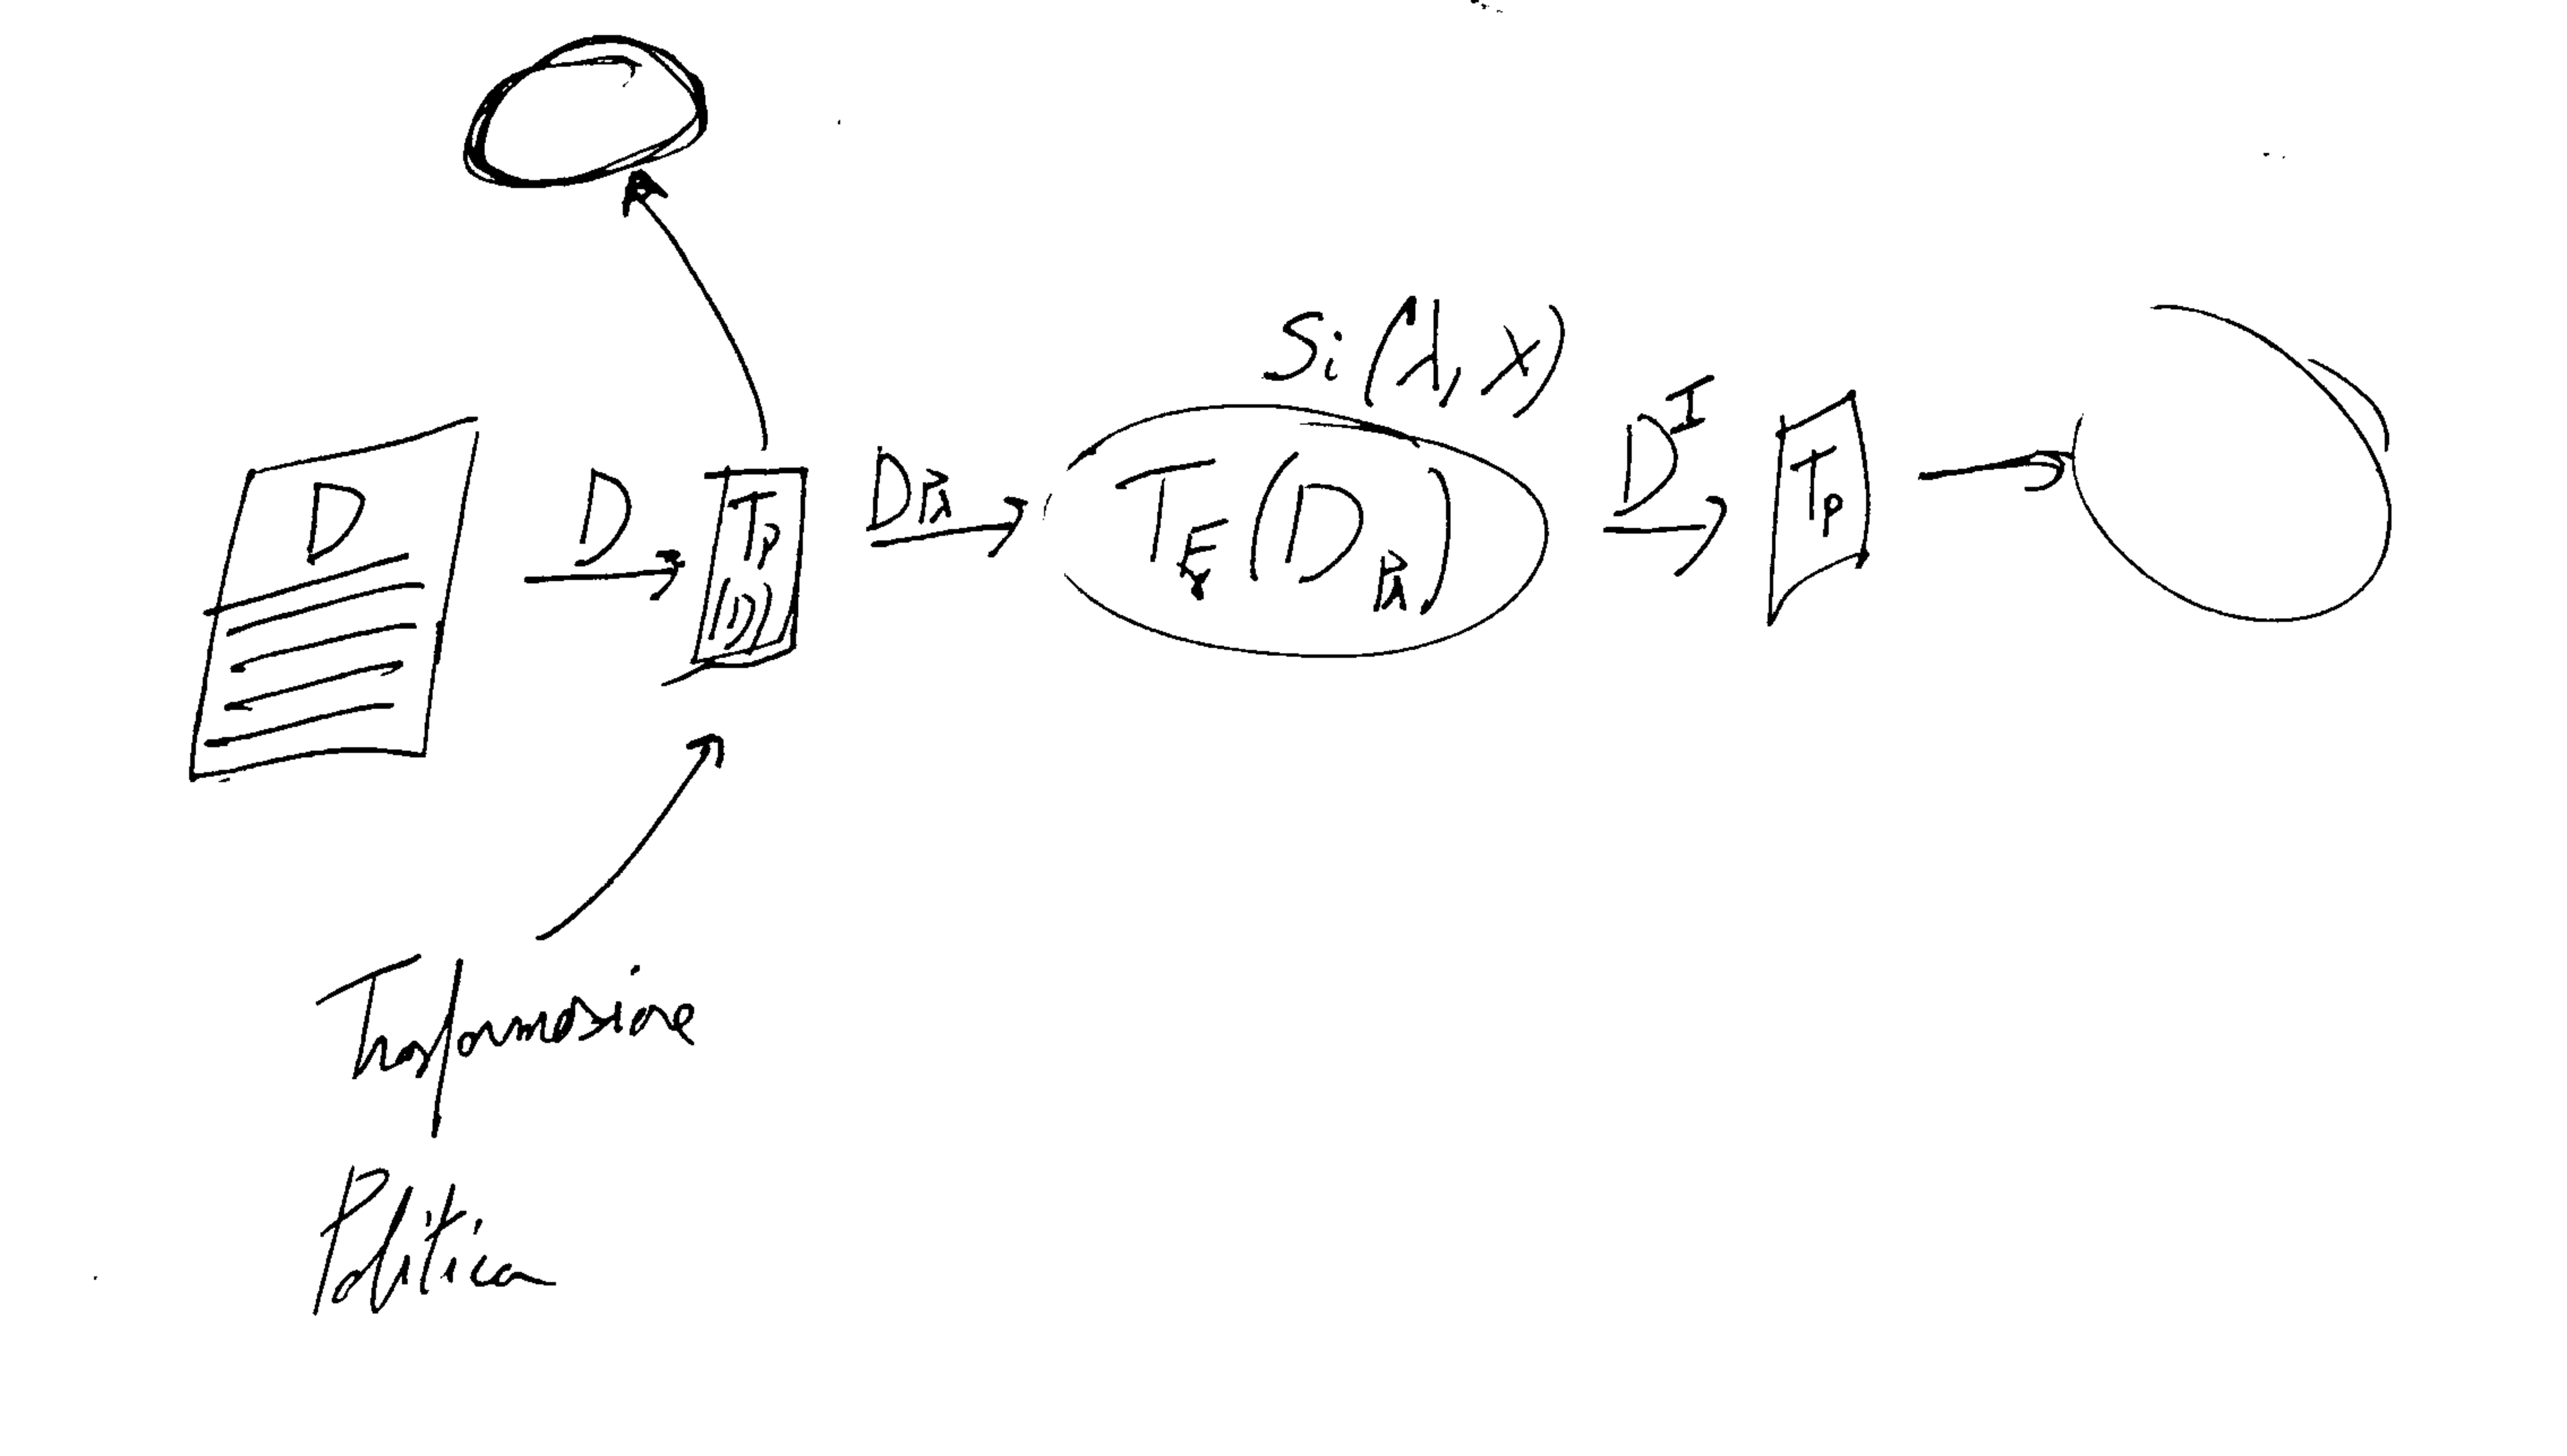
\includegraphics[width=\columnwidth]{serviceDetail.pdf}
  \caption{Service Detail}
  \label{fig:service_detail}reinstall remote-ssh
\end{figure}
